\documentclass[11pt]{iopart}
%Uncomment next line if AMS fonts required
%\usepackage{iopams}
\usepackage{fancyhdr}
\usepackage{graphicx}
\usepackage{todonotes}
\usepackage{subfig}
\usepackage{ulem}
\usepackage{amssymb}
\usepackage{multicol}

\usepackage[hidelinks]{hyperref}
\hypersetup{colorlinks=false}

\pagestyle{fancy}
\lhead{Diffusion Limited Aggregation}
\rhead{Candidate Number: 21594}

\begin{document}

%Makes TODO notes format properly in margin
\setlength{\marginparwidth}{1.5cm}

\title[]{The Ising Model}

\author{Candidate Number: 21594}

\address{Department of Physics,
University of Bath, Bath BA2 7AY, United Kingdom}
\begin{abstract}
TODO
\end{abstract}

%\listoftodos

%Uncomment for PACS numbers title message
%\pacs{00.00, 20.00, 42.10}
% Keywords required only for MST, PB, PMB, PM, JOA, JOB? 
%\vspace{2pc}
%\noindent{\it Keywords}: Article preparation, IOP journals
% Uncomment for Submitted to journal title message
%\submitto{\JPA}
% Comment out if separate title page not required
%\maketitle

\section*{Preface}
Although the coursework was initially presented as a C++ project, I took the liberty of rewriting the Ising Model system in a programming language called Google Go (https://golang.org). The motivation for this is Go has been designed to accommodate systems with high concurrency. This means that instead of simulating 1 system at a time, 10,000 different systems can be simulated simultaneously in different threads. This greatly increases time efficiency and has allowed me to achieve a significant level of statistical significance in my ensemble averages. Furthermore, this has also allowed me to use ergodicity to calculate time averages for the same system with many different values of beta at the same time. The source code for my implementation is accessible on Github: \url{http://tiny.cc/brb75y}.

\section{Introduction and Computational Method}
Ferromagnetism is the property of a material to exhibit speontaneous magnetisation in the absence of an external magnetic field. The Ising Model is a mathematical model that uses the results of thermodynamics and statistical mechanics to describe how magnetic structure in some metals leads to ferromagnetism.

In the Ising Model presented in this paper, a magnetic material is modelled by a regular $N$ x $N$ dimensional square lattice $\Pi$. A given grid point on this lattice $\pi_{(i,j)} \in \Pi$ is indexed by cartesian coordinates $(i, j)$ where $i, j \in [0, N]$. These coordinates are not strictly unique as periodic boundary conditions are applied so that a closed system is modelled. This is to say the grid follows the mappings $(i + \Lambda_i N, j + \Lambda_j N) \to (i, j)$ for $\Lambda_i, \Lambda_j \in \mathbb{Z}$. Each grid point $\pi_{(i, j)} \in \Pi$ on this square lattice is assigned a discrete variable  $s_{(i, j)} \in \{0, 1\}$ that corresponds to the spin of the grid point. We arbitrarily define $s_{(i, j)} = 1$ to represent 'spin up' and $s_{(i,j)} = -1$ to represent 'spin down'.

For a given grid point $\pi_{(i, j)}$, the convention of nearest neighbours is defined as representing the grid points directly adjacent to the grid point, both vertically and horizontally. Using this convention, the energy of a given spin on the grid is defined by
\begin{equation}
E_{(i, j)} = -h_{(i, j)} s_{(i, j)}
\end{equation}
where
\begin{equation}
h_{(i, j)} = \sum_{(\alpha, \beta) \; \textrm{\small{n.n. of}} \; (i, j)} \left[ J  s_{(\alpha, \beta)} \right]
\end{equation}
Here "n.n" represents a sum over the nearest neighbours and $J$ is a positive real number that indicates the strength of the interactions between spins. Qualitatively this set of equations defines the energy of a given spin as the sum of the interaction energies between the spin and it's nearest neighbours, where the interaction energy between two nearest neighbour spins is defined to be $-J$ if the two spins are aligned and $-J$ if the two spins are antiparallel.

\section{Method}

\subsection{Random Walks and Ensemble Averaging}

\subsection{Determining the Fractal Dimension of DLA Aggregates}

\section{Results}

\subsection{Convergence to Equilibrium}

\begin{figure}[t]
  \centering
  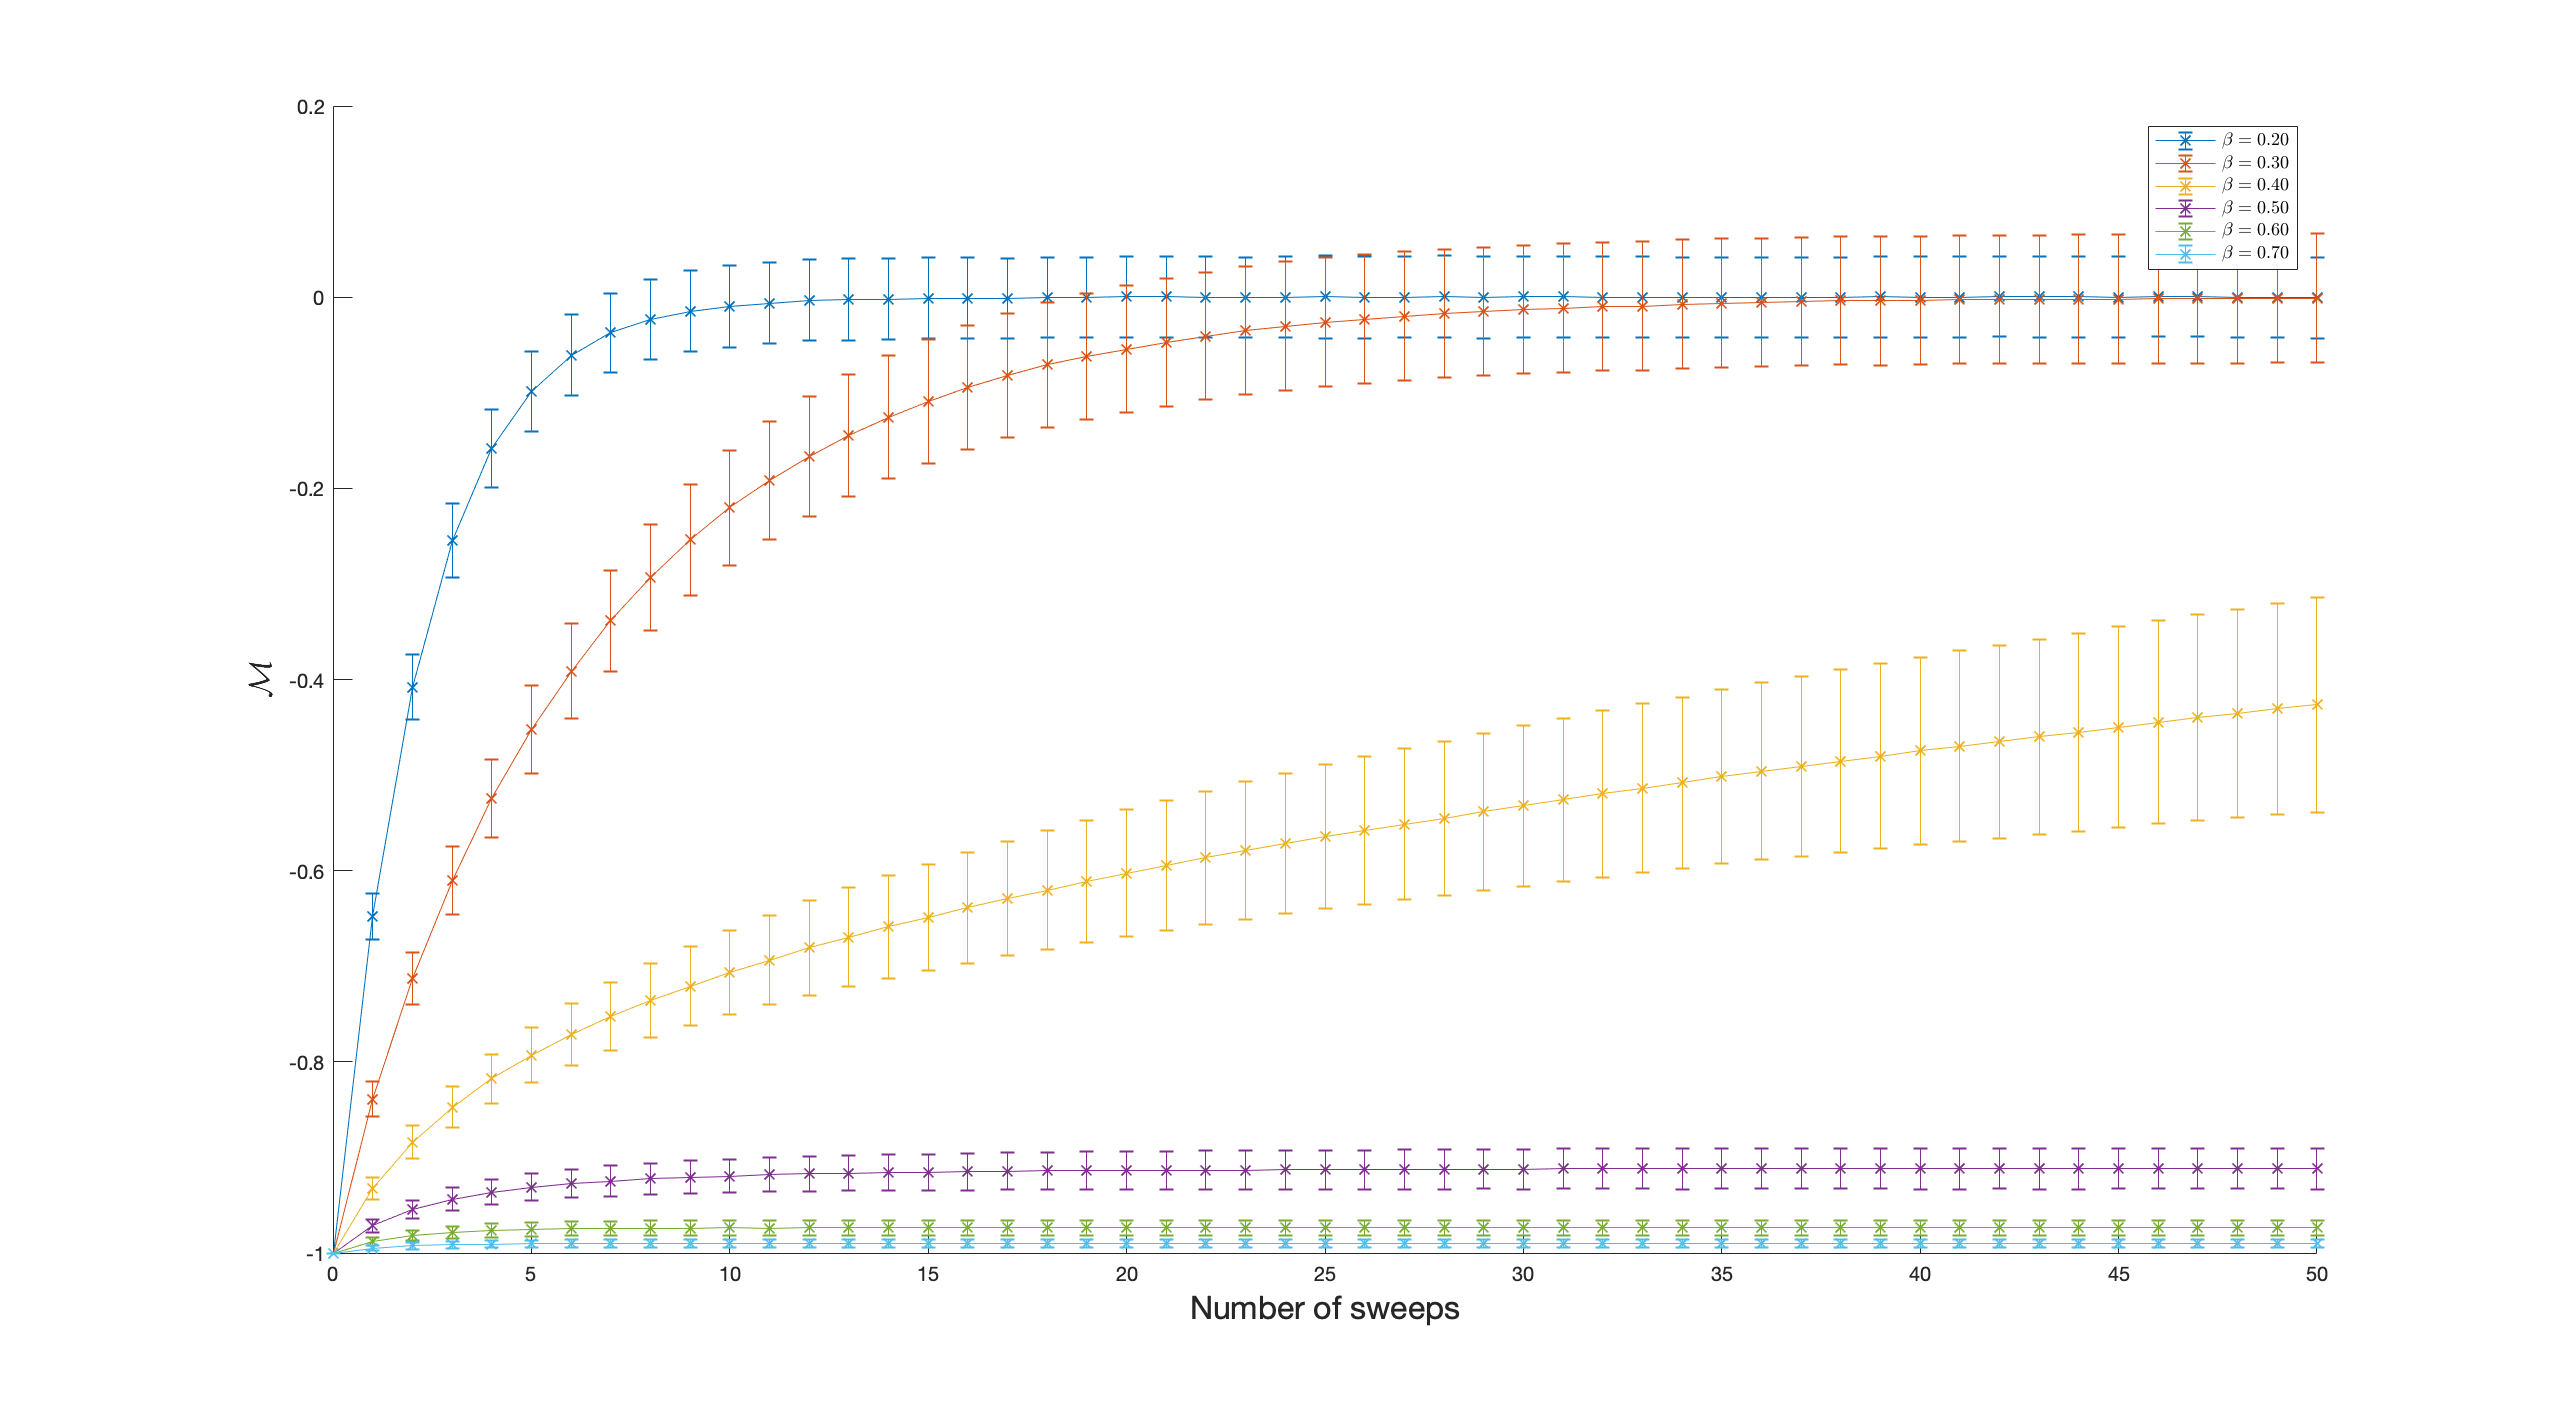
\includegraphics[width=\linewidth]{images/section1/magnetisation.png}
  \caption{Convergence to equilibrium}
  \label{fig:magnetisationsection1}
\end{figure}

\begin{figure}[t]
  \centering
  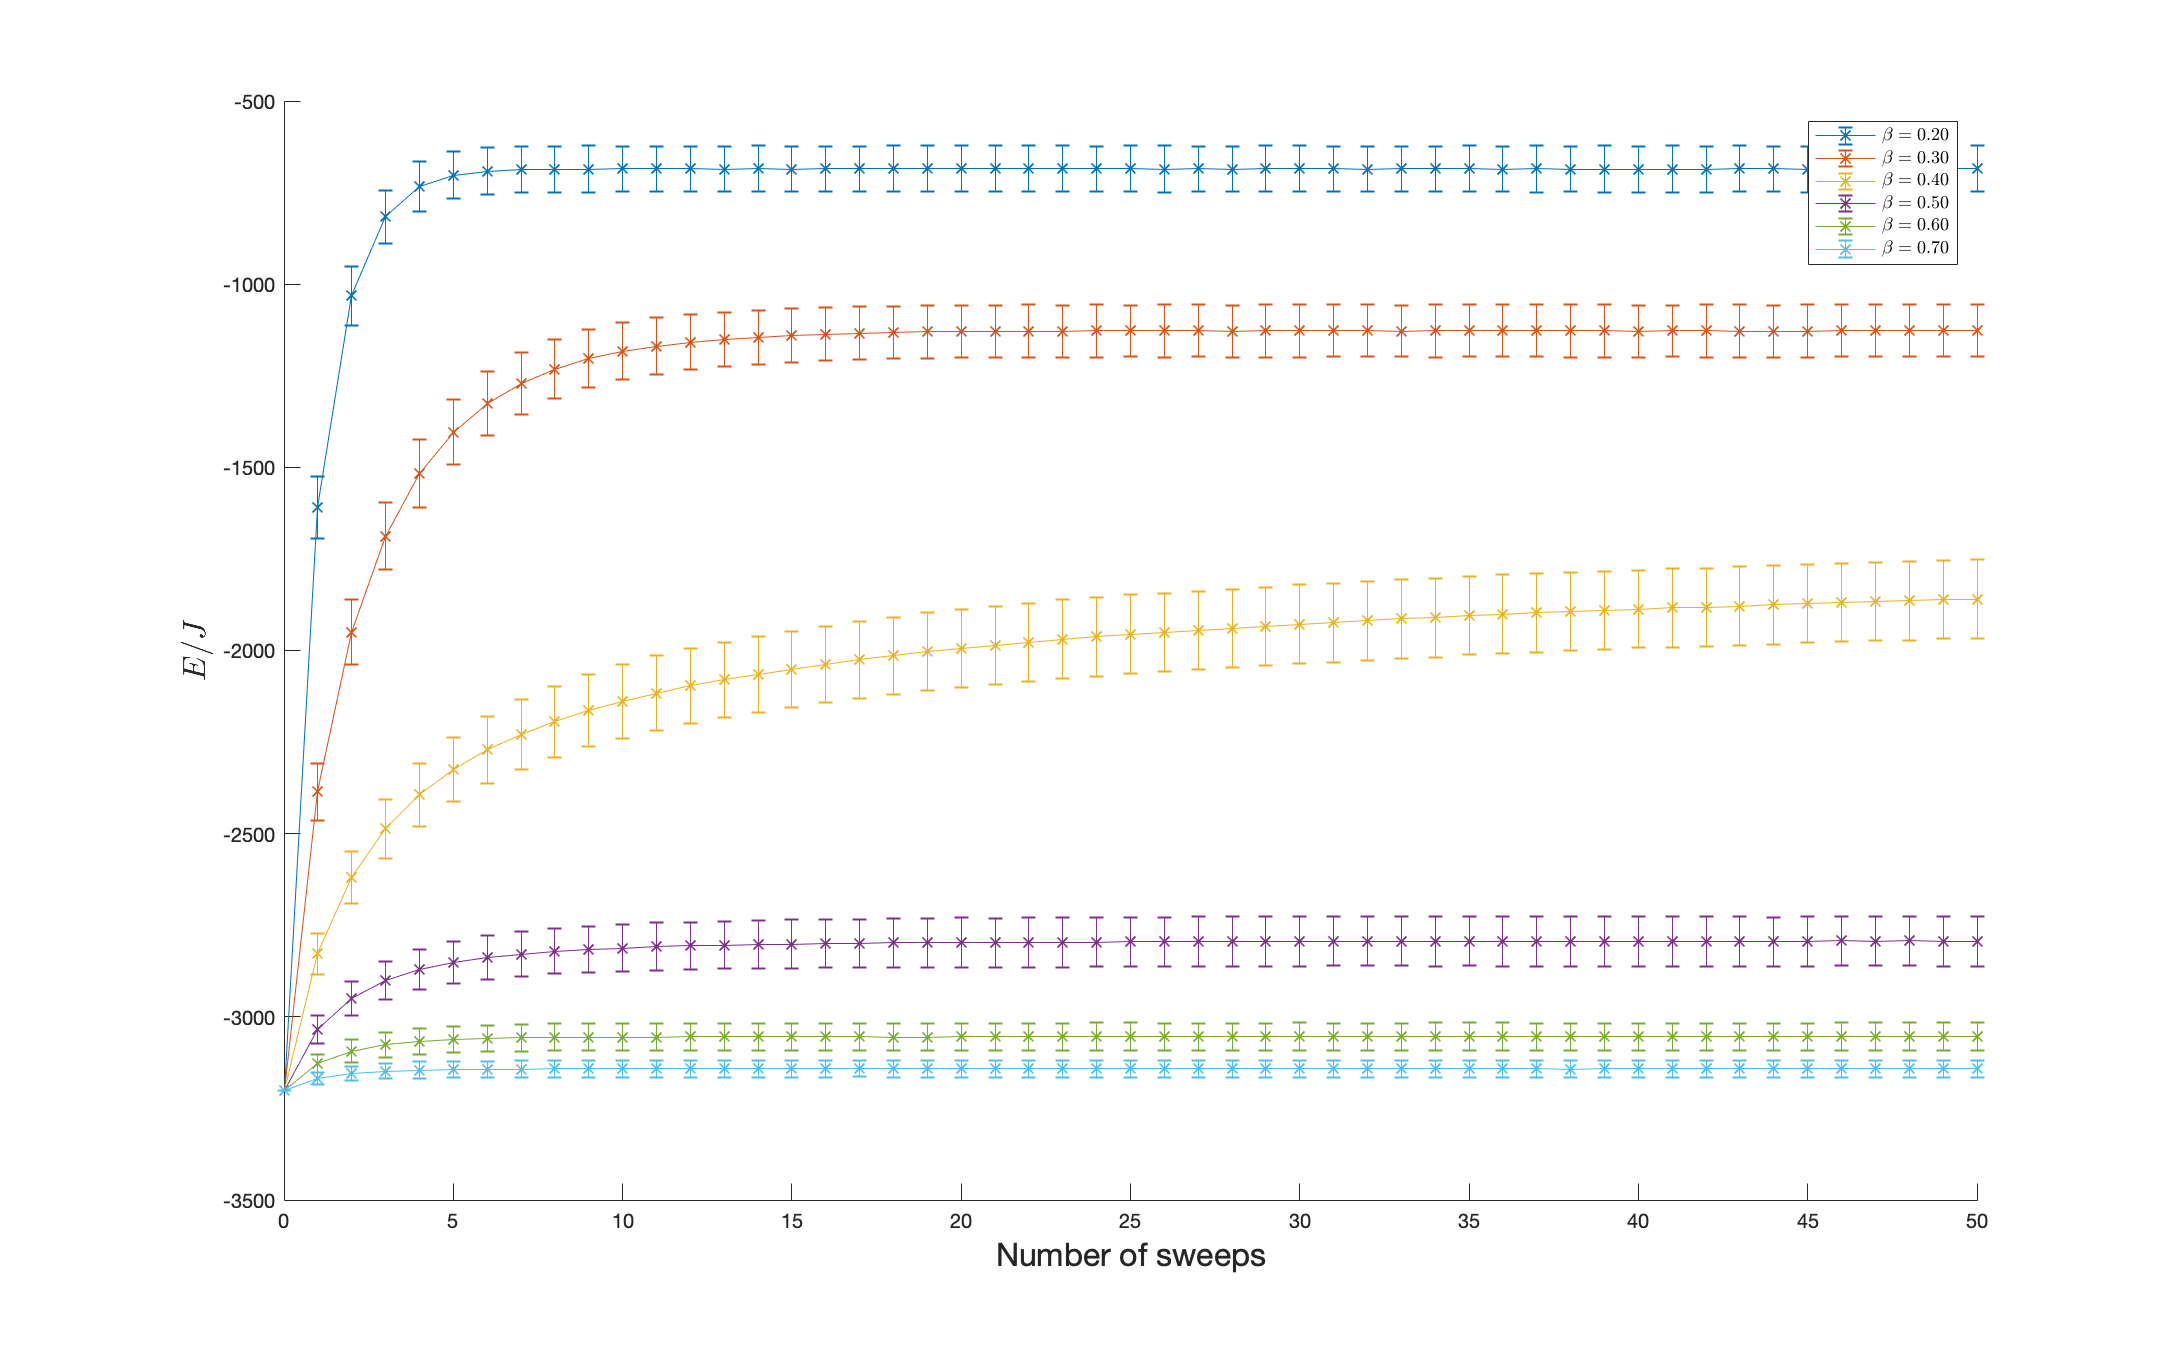
\includegraphics[width=\linewidth]{images/section1/energy.png}
  \caption{Convergence to equilibrium}
  \label{fig:energysection1}
\end{figure}

\subsection{Measuring Equilibrium Averages}

\begin{figure}[t]
  \centering
  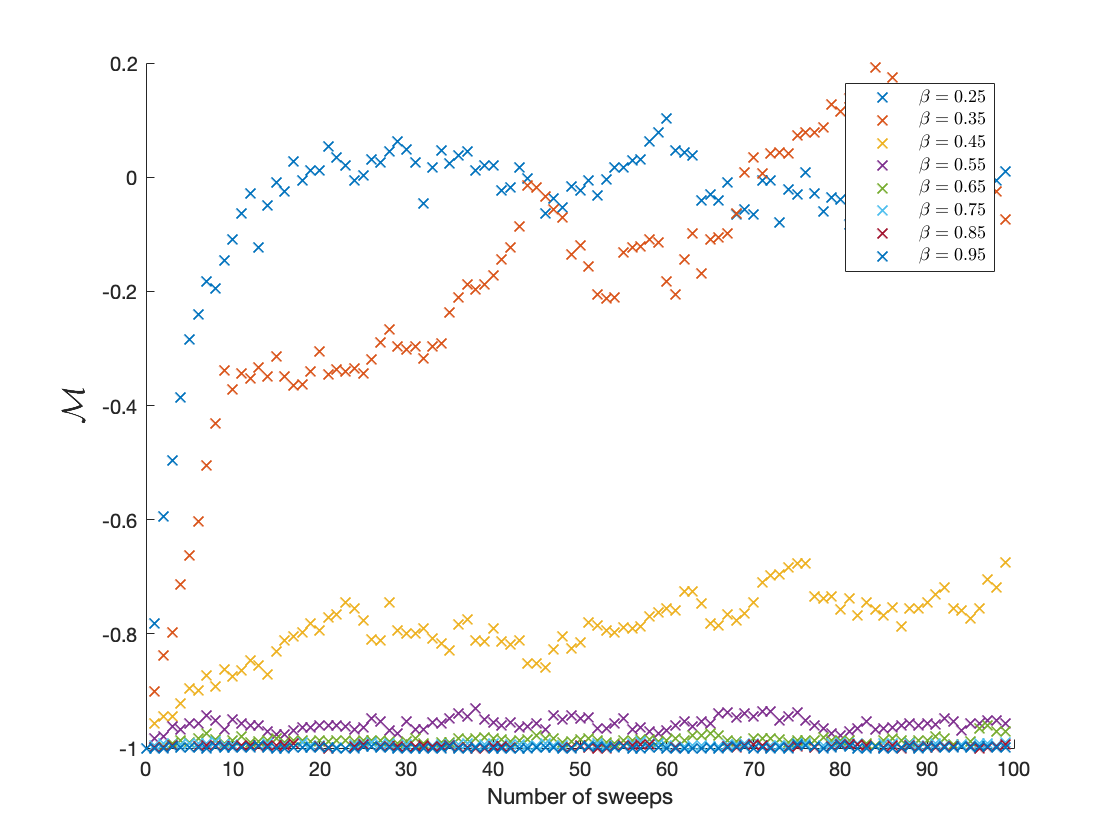
\includegraphics[width=\linewidth]{images/section2/transients.png}
  \caption{Transient behaviour of system}
  \label{fig:transients}
\end{figure}

\section{Discussion}
\subsection{Determining the Fractal Dimension of DLA Aggregates where $p_{stick} = 1$}
\subsection{Suggestions for Improvement}


\section{Conclusion}

\section*{References}
\bibliography{refs}
\bibliographystyle{plain}

\end{document}

